\documentclass{article}
\usepackage{graphicx} % Required for inserting images
\usepackage{authblk}  % For author affiliations

\usepackage{amsmath} % for displaying equations

\usepackage{graphicx}
% \usepackage{amsmath} % For \textmu
\usepackage{booktabs} % For \toprule, \midrule, \bottomrule
\usepackage{float} % For [H] table/figure placement
\usepackage{caption} % For subfigure captions
\usepackage{subcaption} % For subfigures
\usepackage{algorithm} % for algorithms
\usepackage{algorithmic} % for algorithms
\usepackage{multirow} % for multi-row tables
\usepackage{tabularx} % resizable table

\usepackage[
  backend=biber,
  citestyle=numeric,
  bibstyle=numeric,  % Change 'apa' to 'numeric' for numbered references
  sorting=none,      % Ensures references are ordered by citation
  defernumbers=true
]{biblatex} % For references and citations
\addbibresource{references.bib}  % Name of your .bib file

  
\title{Optimized Partitioning for Parallel Sorting in Distributed Heterogeneous Clouds}

\author[]{Joeniño Cainday}
\author[]{Junar Landicho}
\affil[]{University of Science and Technology of Southern Philippines, Cagayan de Oro, 9000, Philippines}

\date{June 2025}

\begin{document}

\maketitle

\begin{abstract}
This study addresses the critical challenge of efficient data partitioning for parallel sorting in distributed, heterogeneous cloud environments.  Simple partitioning schemes often fail in such settings, where nodes have varying processing capabilities, memory capacities, and costs, leading to performance bottlenecks and resource inefficiency.  We propose a novel algorithm, Heterogeneous Parallel Sorting by Linear Programming (H-PSLP), that formulates the partitioning problem as a multi-objective optimization problem.  The H-PSLP model uses a linear program to determine the optimal data allocation, minimizing both execution time (makespan) and monetary cost while strictly adhering to each node's memory constraints. 

A comprehensive simulation-based evaluation was conducted, comparing H-PSLP against a state-of-the-art baseline, H-PSRS, across 54 different configurations, including varying dataset sizes, node counts, and data distributions.  The results demonstrate the definitive superiority of our proposed method. On average, H-PSLP reduces the makespan by 46.3\% and total cost by 69.5\%.  Most critically, it resolves the fundamental instability of the memory-blind baseline, maintaining an average peak memory utilization of 97.6\% compared to the baseline's catastrophic 9,522.3\%, thereby guaranteeing system reliability.  The findings conclude that an upfront, optimization-driven partitioning strategy is significantly more robust and efficient for parallel sorting in heterogeneous systems than traditional heuristic approaches. 
\end{abstract}

\vspace{3em}

\section{Introduction}

The widespread adoption of cloud computing has underscored the importance of efficient resource allocation in distributed systems. Recent literature highlights the rapid growth of cloud adoption across industry sectors. For example, a 2024 survey notes that ``the widespread adoption of cloud computing has dramatically altered how data is stored, processed, and accessed,'' with organizations increasingly relying on cloud services \cite{gptclaim1}. Economic analyses further report that ``the use of the cloud has grown tremendously,'' with capital expenditures by major providers expanding at an unprecedented rate \cite{gptclaim2}. These trends underscore the massive scale and impact of cloud adoption.

However, simple partitioning schemes such as uniform splits or round-robin assignments often perform poorly in heterogeneous environments. Studies in graph analytics on mixed-power clusters reveal that many frameworks assume uniform node performance, leading to imbalances: faster nodes finish early while slower ``straggler'' nodes delay synchronization, thereby increasing the overall makespan \cite{gptclaim7_8}. One such survey on graph partitioning notes that static uniform partitioning causes high-performance machines to remain idle, waiting for slower ones to finish, introducing ``huge processing inefficiencies'' \cite{gptclaim7_8}.

These challenges are further amplified when data is distributed across geographically dispersed nodes. Differences in hardware capabilities, along with increased communication overhead, contribute to latency and reduced system performance \cite{yoon_optimal_2014}. Load balancing is widely recognized as a critical issue in distributed heterogeneous systems. For example, an ACM conference study highlights that ``load-balancing algorithms play a key role in improving the performance of practical distributed systems that consist of heterogeneous nodes'' \cite{gptclaim5}. The difficulty of evenly distributing workloads across nodes with varying capabilities often leads to severe performance degradation due to straggler effects. Recent edge computing research reinforces this point, noting that ``heterogeneity is inevitable... such environments often consist of diverse devices,'' and that achieving balanced workloads across such devices is a significant challenge \cite{gptclaim6}. Thus, load balancing is essential for maintaining system scalability and throughput in heterogeneous environments.

Memory limitations also play a vital role in partitioning. Several recent studies emphasize that data partitions must fit within each node’s memory. For instance, a 2024 ICPP paper on mapping large DAG workflows addresses ``memory-constrained partitioning and mapping of DAG-shaped workflows onto heterogeneous platforms, where each processor can have a different memory size'' \cite{gptclaim14_15}. The authors stress that memory constraints are ``mostly ignored in the literature,'' highlighting the need to include them for correctness \cite{gptclaim14_15}. In practice, a partition that exceeds a node’s memory cannot be executed. Therefore, modern partitioning strategies often model per-node memory capacity as a constraint, as memory availability significantly influences how data or tasks can be allocated.

Beyond performance, cost has emerged as a central factor in partitioning decisions due to the pay-as-you-go nature of modern cloud platforms. Cloud services typically employ usage-based pricing models. Policy studies and technical reviews confirm that cloud platforms offer on-demand access with flexible scalability and charge users based on actual resource usage \cite{gptclaim3, gptclaim4}. For instance, the OECD characterizes cloud services by ``on-demand availability, flexible scalability, and a pay-as-you-go pricing model based on usage and time'' \cite{gptclaim3}. Similarly, Amazon EC2 documentation and academic discussions note that billing is proportional to the amount of resource-time consumed \cite{gptclaim4}. This usage-based model is the standard in Infrastructure-as-a-Service (IaaS) clouds.

While premium instances may offer enhanced performance, their actual capabilities can vary widely across providers. As such, a high-tier instance from one vendor may be comparable to a mid-tier instance from another. Because different instance types exhibit varied price/performance trade-offs, resource allocation strategies must be cost-aware. For example, Stratus, a 2018 study on container scheduling on AWS, demonstrates that ``Stratus’s scale-out decisions are also designed to exploit both instance type diversity and instance pricing variation'' \cite{gptclaim10}. The authors argue that minimizing costs requires jointly deciding how many tasks to assign per server and which instance types to use, based on cost per unit of resource \cite{gptclaim10}. Practical schedulers therefore incorporate instance pricing into allocation strategies, preferring cheaper instance types or spot/preemptible resources when suitable.

Ideally, partitioning decisions should lie on the Pareto frontier—where no improvement in one objective (e.g., cost) can be achieved without degrading another (e.g., speed) \cite{yoon_optimal_2014}. Inefficient partitioning can lead to unnecessary expenses or system failures, such as memory overflows. Therefore, effective solutions must balance these competing objectives.

This study addresses the problem of static data partitioning for parallel sorting in resource-constrained distributed environments. To model node heterogeneity, we account for variations in usage cost, memory capacity, and processing capability. Specifically, we abstract the combined effects of computation speed, communication latency, and bandwidth into a unified performance metric, defined as the relative throughput of each node. For example, a node with twice the throughput of another can process and communicate data approximately twice as fast. In practice, this performance metric ($\text{Perf}[i]$) can be estimated via benchmarking or analysis of historical performance logs.

To solve this multi-objective optimization problem, we propose a linear programming (LP) approach that produces cost-aware and load-balanced data partitioning strategies. The model minimizes both execution time (makespan) and total resource cost, while ensuring compliance with memory constraints. Unlike heuristic or sampling-based methods, the LP formulation guarantees globally optimal solutions under linear constraints. 

\vspace{3em}

\section{Review of Related Research}


In the domain of parallel sorting, many algorithms operate under the assumption of a homogeneous computing environment. For instance, Parallel Sorting by Regular Sampling (PSRS) selects pivots to divide the dataset into equally sized partitions \cite{tokuue_fugaku_2023}, and commonly used benchmarks are based on synthetically generated data with uniform or otherwise idealized distributions. However, such methods often fail to account for the heterogeneity inherent in real-world distributed systems. Addressing this limitation, \cite{monga_parallel_heterogeneous} introduced a modified version of PSRS designed for heterogeneous environments. Their approach improves load balancing by allocating data in proportion to each node's relative performance. However, their method overlooks several critical system attributes and exhibits multiple issues, as discussed in Section~\ref{sec:methodology}.

In the context of distributed systems, this research distinguishes itself from existing works such as \cite{yoon_optimal_2014} by adopting a more focused approach tailored to parallel sorting. While that study tackles optimal dataset allocation across geographically distributed cloud data centers using a multi-objective linear programming (LP) model to generate a Pareto front minimizing both processing time and monetary cost, our research employs a scalarized LP objective focused on minimizing makespan, with cost incorporated as a weighted factor. This formulation allows for a direct and computationally efficient solution specific to data partitioning in heterogeneous nodes. It also simplifies complex inter-node considerations such as communication and transfer speeds by abstracting them into a generalized “throughput” metric, which encapsulates latency, bandwidth, and computation speed — making it practical for parallel sorting tasks.

In big-data systems like Apache Spark, dynamic partitioning and scheduling algorithms have also been proposed. For example, \cite{lu_time_aware_2023} developed a dynamic partitioning strategy for intermediate Spark data to mitigate skew, along with a greedy scheduling method that considers node speed. Their results show that balanced partitioning significantly reduces completion time. Our work differs by focusing on static initial partitioning using explicit node metrics, rather than runtime rebalancing.

Linear and mixed-integer programming has been applied to heterogeneous data partitioning in other domains, though not specifically for sorting. \cite{gptlp3} formulate query execution on a heterogeneous cluster as an LP problem, measuring each node's performance and using optimization to generate a recommended data partitioning scheme. This “resource bricolage” approach balances workload across fast and slow machines. \cite{gptlp4_5} consider hybrid CPU/GPU systems and construct a mixed-integer LP model for data assignment, scheduling a large number of parallel data chunks to minimize execution time. \cite{gptlp6} tackle task graphs on geo-distributed heterogeneous systems, proposing two MILP-based strategies to minimize the execution time of dataflow-driven tasks. Similarly, \cite{gptlp7} use an LP model ("Tetrium" scheduler) for multi-resource scheduling in heterogeneous datacenters. More recently, \cite{gptlp8} apply LP to heterogeneous sequence parallelism for LLM training, modeling the problem as a linear optimization and designing a solver to assign variable-length sequences across GPUs and CPUs. These examples demonstrate that LP/MILP is well-established for balancing workloads in heterogeneous environments. However, none of these works address the problem of sorting. Instead, they focus on queries, general data-parallel tasks, or scheduling.

The use of Linear Programming for static partitioning in the specific context of parallel sorting appears to be novel. All reviewed heterogeneous sorting papers employ other techniques. Prior work has focused on analytical models or sampling-based heuristics. For instance, \cite{gptlp1} propose sampling and dynamic programming approaches to balance load via proportional partitioning, while \cite{gptlp2} introduce heterogeneity-aware variants of sample-sort and over-partitioning (H-PSRS and H-PSOP). These methods achieve excellent balance (imbalance within 0.1\% or 0.01\% of ideal), using pivot sampling and oversampling techniques. Lastovetsky and Reddy (2004/2006) developed closed-form and DP solutions based on functional performance models. Cérin et al. explicitly note that a “divisible load” linear model, such as those by Drozdowski et al., does not apply to sorting due to non-linear merging costs (as cited in \cite{gptlp1}). In contrast, our approach encodes partition sizes explicitly in an LP and solves for optimal balance based on the nodes’ specifications. While it shares conceptual similarities with the aforementioned LP-based strategies, those works address different computational problems.


\section{Methodology}
\label{sec:methodology}

This section details the design and rationale behind the proposed Heterogeneous Parallel Sorting by Linear Programming (H-PSLP) algorithm. To establish a clear performance baseline, we first analyze the operational and complexity-related shortcomings of a state-of-the-art heterogeneous sorting algorithm, H-PSRS. We then present H-PSLP as a redesigned approach that directly addresses these limitations through mathematical optimization, leading to a more efficient, cost-aware, and reliable sorting process.

\begin{figure}[H]
    \centering
    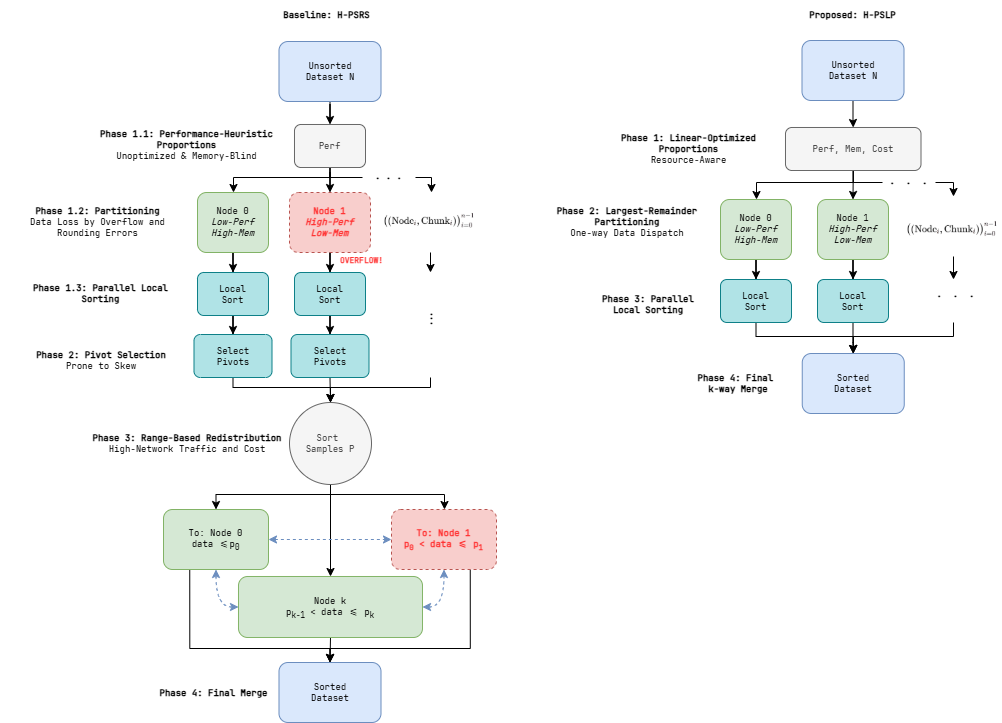
\includegraphics[width=1\linewidth]{images/workflow.png}
    \caption{Architectural Comparison: The multi-stage, communication-heavy workflow of H-PSRS (left) versus the streamlined, optimization-first workflow of H-PSLP (right). H-PSLP avoids memory overflows, eliminates all-to-all communication, and reduces redundant sorting.}
    \label{fig:workflow_comparison}
\end{figure}

The H-PSLP workflow, outlined in Algorithm~\ref{alg:hpslp}, begins with its core innovation: a Linear Programming (LP) optimization phase. Instead of heuristically partitioning data, the coordinator node solves an LP model that considers the entire system's state—each node's throughput, memory capacity, and billing rate—to determine a globally optimal data allocation. This crucial first step ensures that data partitions are sized not only for balanced execution time but also to prevent memory overflows and reduce cost from the outset. Following this optimization, H-PSLP's structure is streamlined. The need for local sampling, centralized pivot selection, and the costly all-to-all data redistribution is entirely obviated. To convert the potentially fractional solution from the LP solver into a discrete integer allocation, we employ the largest remainder method (also known as Hamilton's method), a classic apportionment algorithm recognized for its effectiveness in proportionally distributing resources~\cite{gptclaim11_12, gptclaim13}. Each node then performs a single, parallel local sort on its optimally assigned data chunk. Finally, Phase IV involves a centralized, efficient $p$-way min-heap merge on the coordinator, a standard and I/O-efficient subroutine used in external and parallel sorting systems~\cite{gptmerge1_2, gptmerge3_7, gptmerge4_5_8}.

This architectural shift not only reduces inter-node communication but also yields significant improvements in computational complexity. The upfront investment in solving the LP model, which has a worst-case time complexity of \( O(p^3) \) using interior-point methods, is quickly offset by the elimination of H-PSRS's more expensive and less scalable phases. Specifically, H-PSLP replaces the \( O(p^2 \log p) \) sampling bottleneck and the \( O(n) \) all-to-all communication overhead with a single global optimization step that depends only on the number of nodes \( p \), not on the dataset size \( n \). In practical large-scale sorting scenarios where \( n \gg p^3 \), the time spent on data-intensive operations—namely the parallel local sort \( O\left(\frac{n \log n}{p}\right) \) and the final centralized merge \( O(n \log p) \)—dominates the total execution time. As a result, the \( O(p^3) \) overhead of the LP solver becomes a negligible fraction of the total makespan, allowing H-PSLP to achieve superior scalability as dataset sizes and node counts grow.



% ----------------- H-PSLP Algorithm -----------------
\begin{algorithm}[H]
\caption{Heterogeneous Parallel Sorting by Linear Programming (H-PSLP)}
\label{alg:hpslp}
\begin{algorithmic}[1]
\REQUIRE Dataset $S$ of size $n$, list of $p$ nodes with their `Performance`, `Memory`, and `Cost` profiles
\ENSURE A single, globally sorted dataset $S'$

\STATE \textbf{Phase I: Optimization (Coordinator Node)}
\STATE Run Linear Programming solver to calculate the optimal partition size $x[i]$ for each node $i$.

\STATE \textbf{Phase II: Data Partitioning (Coordinator Node)}
\STATE Convert potentially fractional $x[i]$ values to integer partition sizes using the largest remainder method.
\STATE Split the dataset $S$ into $p$ chunks $C_0, C_1, \dots, C_{p-1}$ based on the calculated integer sizes.
\STATE Distribute each chunk $C_i$ to its corresponding node $N_i$.

\STATE \textbf{Phase III: Parallel Local Sorting (All Nodes)}
\FOR{each node $N_i$ from $0$ to $p-1$ \textbf{in parallel}}
    \STATE Perform a local sort on the assigned data chunk $C_i$.
    \STATE Send the sorted chunk back to the coordinator.
\ENDFOR

\STATE \textbf{Phase IV: Final Merge (Coordinator Node)}
\STATE Coordinator collects all sorted chunks from the nodes.
\STATE Perform a $p$-way merge on the sorted chunks using a min-heap to create the final sorted dataset $S'$.
\RETURN $S'$
\end{algorithmic}
\end{algorithm}

\subsubsection{Linear Programming Formulation}
\label{sec:lp_formulation}

The intelligence of H-PSLP is encapsulated in its LP formulation, which seeks an optimal workload allocation that minimizes a scalarized objective combining makespan and monetary cost. This formulation models the system's primary constraints, ensuring a robust and efficient solution.

\begin{align}
\text{minimize} \quad & T + \lambda \sum_{i=0}^{p-1} \text{Cost}[i] \cdot \frac{x[i] \cdot \beta}{\text{Perf}[i]} \label{eq:objective}\\
\text{subject to} \quad & \sum_{i=0}^{p-1} x[i] = n \label{eq:workload_constraint}\\
& x[i] \leq \text{Mem}[i] \quad \forall i \in \{0, \ldots, p-1\} \label{eq:memory_constraint}\\
& T \geq \frac{x[i] \cdot \beta}{\text{Perf}[i]} \quad \forall i \in \{0, \ldots, p-1\} \label{eq:makespan_constraint}\\
& x[i] \geq 0 \quad \forall i \in \{0, \ldots, p-1\} \label{eq:non_negative}
\end{align}

Here, the decision variable $x[i]$ represents the number of data items assigned to node $i$, and $T$ represents the makespan, or the maximum completion time across all nodes. The objective function~\eqref{eq:objective} aims to minimize the makespan $T$, while also considering the total monetary cost. The parameter $\lambda$ allows for tuning the trade-off between time and cost, and $\beta$ is a factor that normalizes the workload to a time unit.

The constraints ensure the validity of the solution. Constraint~\eqref{eq:workload_constraint} ensures that all data is allocated. Critically, constraint~\eqref{eq:memory_constraint} explicitly enforces each node's memory capacity, directly preventing the memory overflow issues that plague the H-PSRS baseline. The makespan constraint~\eqref{eq:makespan_constraint} defines $T$ as the maximum of all individual node processing times, which are modeled as being inversely proportional to their respective throughputs. Finally, constraint~\eqref{eq:non_negative} ensures that all data allocations are non-negative. By solving this model, H-PSLP achieves a globally optimal partitioning scheme under the given linear assumptions, a significant advantage over heuristic-based approaches.



\section{Experimental Setup}

This section describes the simulation framework, cluster configurations, dataset generation, performance metrics, and experimental procedures used to evaluate the proposed H-PSLP algorithm against the H-PSRS baseline.

\subsection{Simulation Environment and Tools}

All experiments were implemented in Python 3 using a custom-built, process-based simulation framework. Parallelism was modeled using Python's \texttt{multiprocessing} module to accurately represent concurrent node operations. The efficient k-way merge phase of the sorting algorithms relied on the \texttt{heapq} library. The core of the H-PSLP algorithm, its LP-based optimization component, was solved using the Google OR-Tools library with the Coin-or branch and cut (CBC) solver. For data generation and visualization, we utilized the \texttt{numpy}, \texttt{matplotlib}, and \texttt{seaborn} libraries.

\subsection{Dataset and Cluster Configuration}

A notable distinction of our experimental design is the handling of data partitioning. Baseline literature on heterogeneous parallel sorting, such as the original H-PSRS paper, employs a Least Common Multiple (LCM) scheme to generate custom dataset sizes that are perfectly divisible across nodes with varying throughputs. This simplifies partitioning but may not reflect real-world scenarios where data sizes are fixed. In contrast, our experiments intentionally use fixed-size datasets to provide a more standardized and realistic benchmark for both algorithms. H-PSRS partitions this data proportionally based on node throughput, while our proposed H-PSLP leverages the Hamilton (largest remainder) method to intelligently apportion data chunks according to the LP solver's optimal fractional solution, ensuring a globally-aware and balanced distribution.

We benchmarked the algorithms using three fixed dataset sizes---$10^4$, $10^5$, and $10^6$ elements---under two distinct data distributions:

\begin{itemize}
    \item \textbf{Uniform distribution} over the integer range $[0, N]$, where $N$ is the dataset size.
    \item \textbf{Gaussian (normal) distribution} with a mean of $\mu = N/2$ and a standard deviation of $\sigma = N/6$. The generated values were clipped to remain within the integer range $[0, N]$.
\end{itemize}

These parameters use a clipped Gaussian distribution to produce a consistent, statistically controlled data skew across all dataset sizes, creating a robust test case for evaluating partitioning effectiveness.

The heterogeneous cluster for each experiment was procedurally generated with the following parameters:

\begin{itemize}
    \item \textbf{Node Throughput (\texttt{Perf[i]}):} Each node's relative processing capability was randomly sampled from the integer range $[1, 10]$.
    \item \textbf{Memory Allocation (\texttt{Mem[i]}):} The total cluster memory was set to 1.5 times the dataset size (\texttt{memory\_overprovision\_factor=1.5}). This total memory was then distributed among the nodes using random fractional weights, creating heterogeneous memory limits for each node.
    \item \textbf{Billing Costs (\texttt{Cost[i]}):} Each node was assigned a billing rate uniformly sampled from the range $[0.1, 1.0]$ arbitrary cost units per unit of simulated time.
\end{itemize}

To ensure comprehensive testing, experiments were conducted across \textbf{2, 5, and 8 nodes}. Each combination of parameters was run with three fixed random seeds (\textbf{4, 5, and 6}) to account for variability in cluster generation and data ordering. This results in a total of 54 unique experimental configurations:
\[
\underbrace{2 \text{ distributions}}_{\text{Uniform, Gaussian}}
\times \underbrace{3 \text{ node counts}}_{2,5,8}
\times \underbrace{3 \text{ dataset sizes}}_{10^4, 10^5, 10^6}
\times \underbrace{3 \text{ seeds}}_{4,5,6} = 54 \text{ runs}
\]

In both H-PSRS and H-PSLP experiments, a designated coordinator (Node 0) handles centralized tasks. To assign this role, the list of generated nodes is sorted in descending order of throughput before the simulation begins, ensuring the node with the highest rating (\texttt{Perf[i]}) typically serves as the coordinator. It is important to note that Node 0 still participates in the parallel sort and is subject to the same constraints as all other nodes for that task. To simplify the coordinator model, we only assume it has sufficient capacity for its additional, coordinator-specific duties (e.g., storing all samples or the final merged list); memory constraints for these specific operations are ignored. The simulated makespan and cost incurred by the coordinator during all its tasks, including both sorting and coordination, are still measured and included in the overall algorithm performance metrics.


\subsection{Heterogeneous Performance Simulation}

To model the performance of a heterogeneous cluster, we first established a \texttt{base\_throughput} by timing a standard sequential sort on the entire dataset. This baseline represents the inverse of processing speed (in microseconds per element) on a notional 1x performance node.

\[
\text{base\_throughput} = \frac{(\text{time\_end\_seq} - \text{time\_start\_seq}) \times 10^6}{N}
\]

For each parallel task (e.g., local sort, merge) in the simulation, the actual wall-clock time of the Python operation was measured. This time was then scaled to produce a simulated delay reflecting the specific throughput of the node executing the task:

\[
\text{simulated\_delay}_{\mu s} = \frac{\text{actual\_time}_{\text{sec}} \times 10^6}{\text{Perf}[i]}
\]

The monetary cost for the task was then calculated by multiplying this simulated delay by the node's billing rate. The \texttt{base\_throughput} was also used by the H-PSLP algorithm's LP solver to predict the makespan for its optimized data distribution.

\subsection{Performance Metrics}

The evaluation focused on several key metrics to provide a holistic view of algorithm performance. For a given algorithm run with $P$ nodes, let $T_{i,j}$ be the simulated time for task $j$ on node $i$, and $C_{i,j}$ be its corresponding cost.

The primary measure of performance is the \textbf{Makespan}, defined as the total execution time of the parallel algorithm, which is determined by the node that finishes last. It is calculated as the maximum of the total simulated time across all nodes:
\[ \text{Makespan} = \max_{i=1}^{P} \left( \sum_{j} T_{i,j} \right). \]
Complementing this is the \textbf{Total Cost}, which represents the cumulative monetary cost incurred across all nodes and all tasks for the duration of the parallel sort, computed as:
\[ \text{Total Cost} = \sum_{i=1}^{P} \sum_{j} C_{i,j}. \]

To assess an algorithm's stability and efficiency in resource-constrained environments, we measure the \textbf{Maximum Peak Memory Utilization}. This metric identifies the highest memory pressure on any single node and is critical for detecting potential memory overflows. A value greater than 100\% indicates that an algorithm assigned more data to a node than its memory capacity allows. Letting $\text{Items}_{i, \text{peak}}$ be the maximum number of data items held in memory by node $i$ during the simulation, it is calculated as:
\[ \text{Max Peak Memory Util} (\%) = \max_{i=1}^{P} \left( \frac{\text{Items}_{i, \text{peak}}}{\text{Mem}[i]} \times 100 \right). \]

Finally, to validate the predictive power of the H-PSLP algorithm, we assess its \textbf{LP Model Accuracy}. It is important to note that the LP model exclusively optimizes the parallel local sort phase; it does not account for subsequent phases like the final centralized merge, nor does it factor in the strategic selection of the coordinator. Therefore, to provide a direct and fair measure of the model's accuracy, we compare the solver's predicted makespan (\texttt{\^{}makespan}) and cost (\texttt{\^{}cost}) against the actual performance of only the local sort phase. The predicted values are compared against the \textbf{Actual Sort Makespan}, which is the time taken by the last node to finish its individual sort task ($T_{i, \text{sort}}$), and the \textbf{Actual Sort Cost}, which is the sum of costs for all individual sort tasks ($C_{i, \text{sort}}$). These are formulated as:
\[ \text{Actual Sort Makespan} = \max_{i=1}^{P} (T_{i, \text{sort}}) \]
\[ \text{Actual Sort Cost} = \sum_{i=1}^{P} C_{i, \text{sort}}. \]
This direct comparison provides a clear measure of the current model's accuracy. Modeling the entire architecture remains a direction for future work.





\section{Results and Analysis}

The empirical results from 54 simulation runs provide a comprehensive comparison between the baseline Heterogeneous Parallel Samplesort (H-PSRS) and our proposed H-PSLP algorithm. The analysis demonstrates that H-PSLP's architecture, centered on a constrained optimization model, delivers substantial and consistent improvements in makespan, cost, and system stability, particularly under conditions of data skew and increasing scale.

\subsection{Overall Performance: Efficiency, Cost, and Stability}

A high-level comparison, averaged across all experimental configurations, reveals the fundamental performance differences between the two algorithms. The aggregated results, summarized in Table~\ref{tab:agg_metrics} and visualized in Figure~\ref{fig:overall_perf}, show that H-PSLP is superior in every key metric.

% --- Table 1: Aggregated Performance Metrics ---
\begin{table}[h!]
\centering
\caption{Aggregated Performance Metrics (Averaged Across All 54 Runs)}
\label{tab:agg_metrics}
\begin{tabularx}{\textwidth}{@{}lXX@{}}
\toprule
\textbf{Metric} & \textbf{H-PSRS} & \textbf{H-PSLP} \\ \midrule
\textbf{Avg. Makespan ($\mu$s)} & 29,645.5 & 15,916.4 \\
\textbf{Avg. Total Cost (\$)} & 47,073.4 & 14,372.9 \\
\textbf{Avg. Max Memory Util. (\%)} & 9,522.3\% & 97.6\% \\
\textbf{Worst-Case Memory Util. (\%)} & 83,330.0\% & 100.1\% \\ \bottomrule
\end{tabularx}
\end{table}


% --- Figure 1: Overall Performance ---
\begin{figure}[h!]
    \centering
    % Ensure the image file 'agg_metrics_comparison.png' is in the same directory
    % or provide the correct path.
    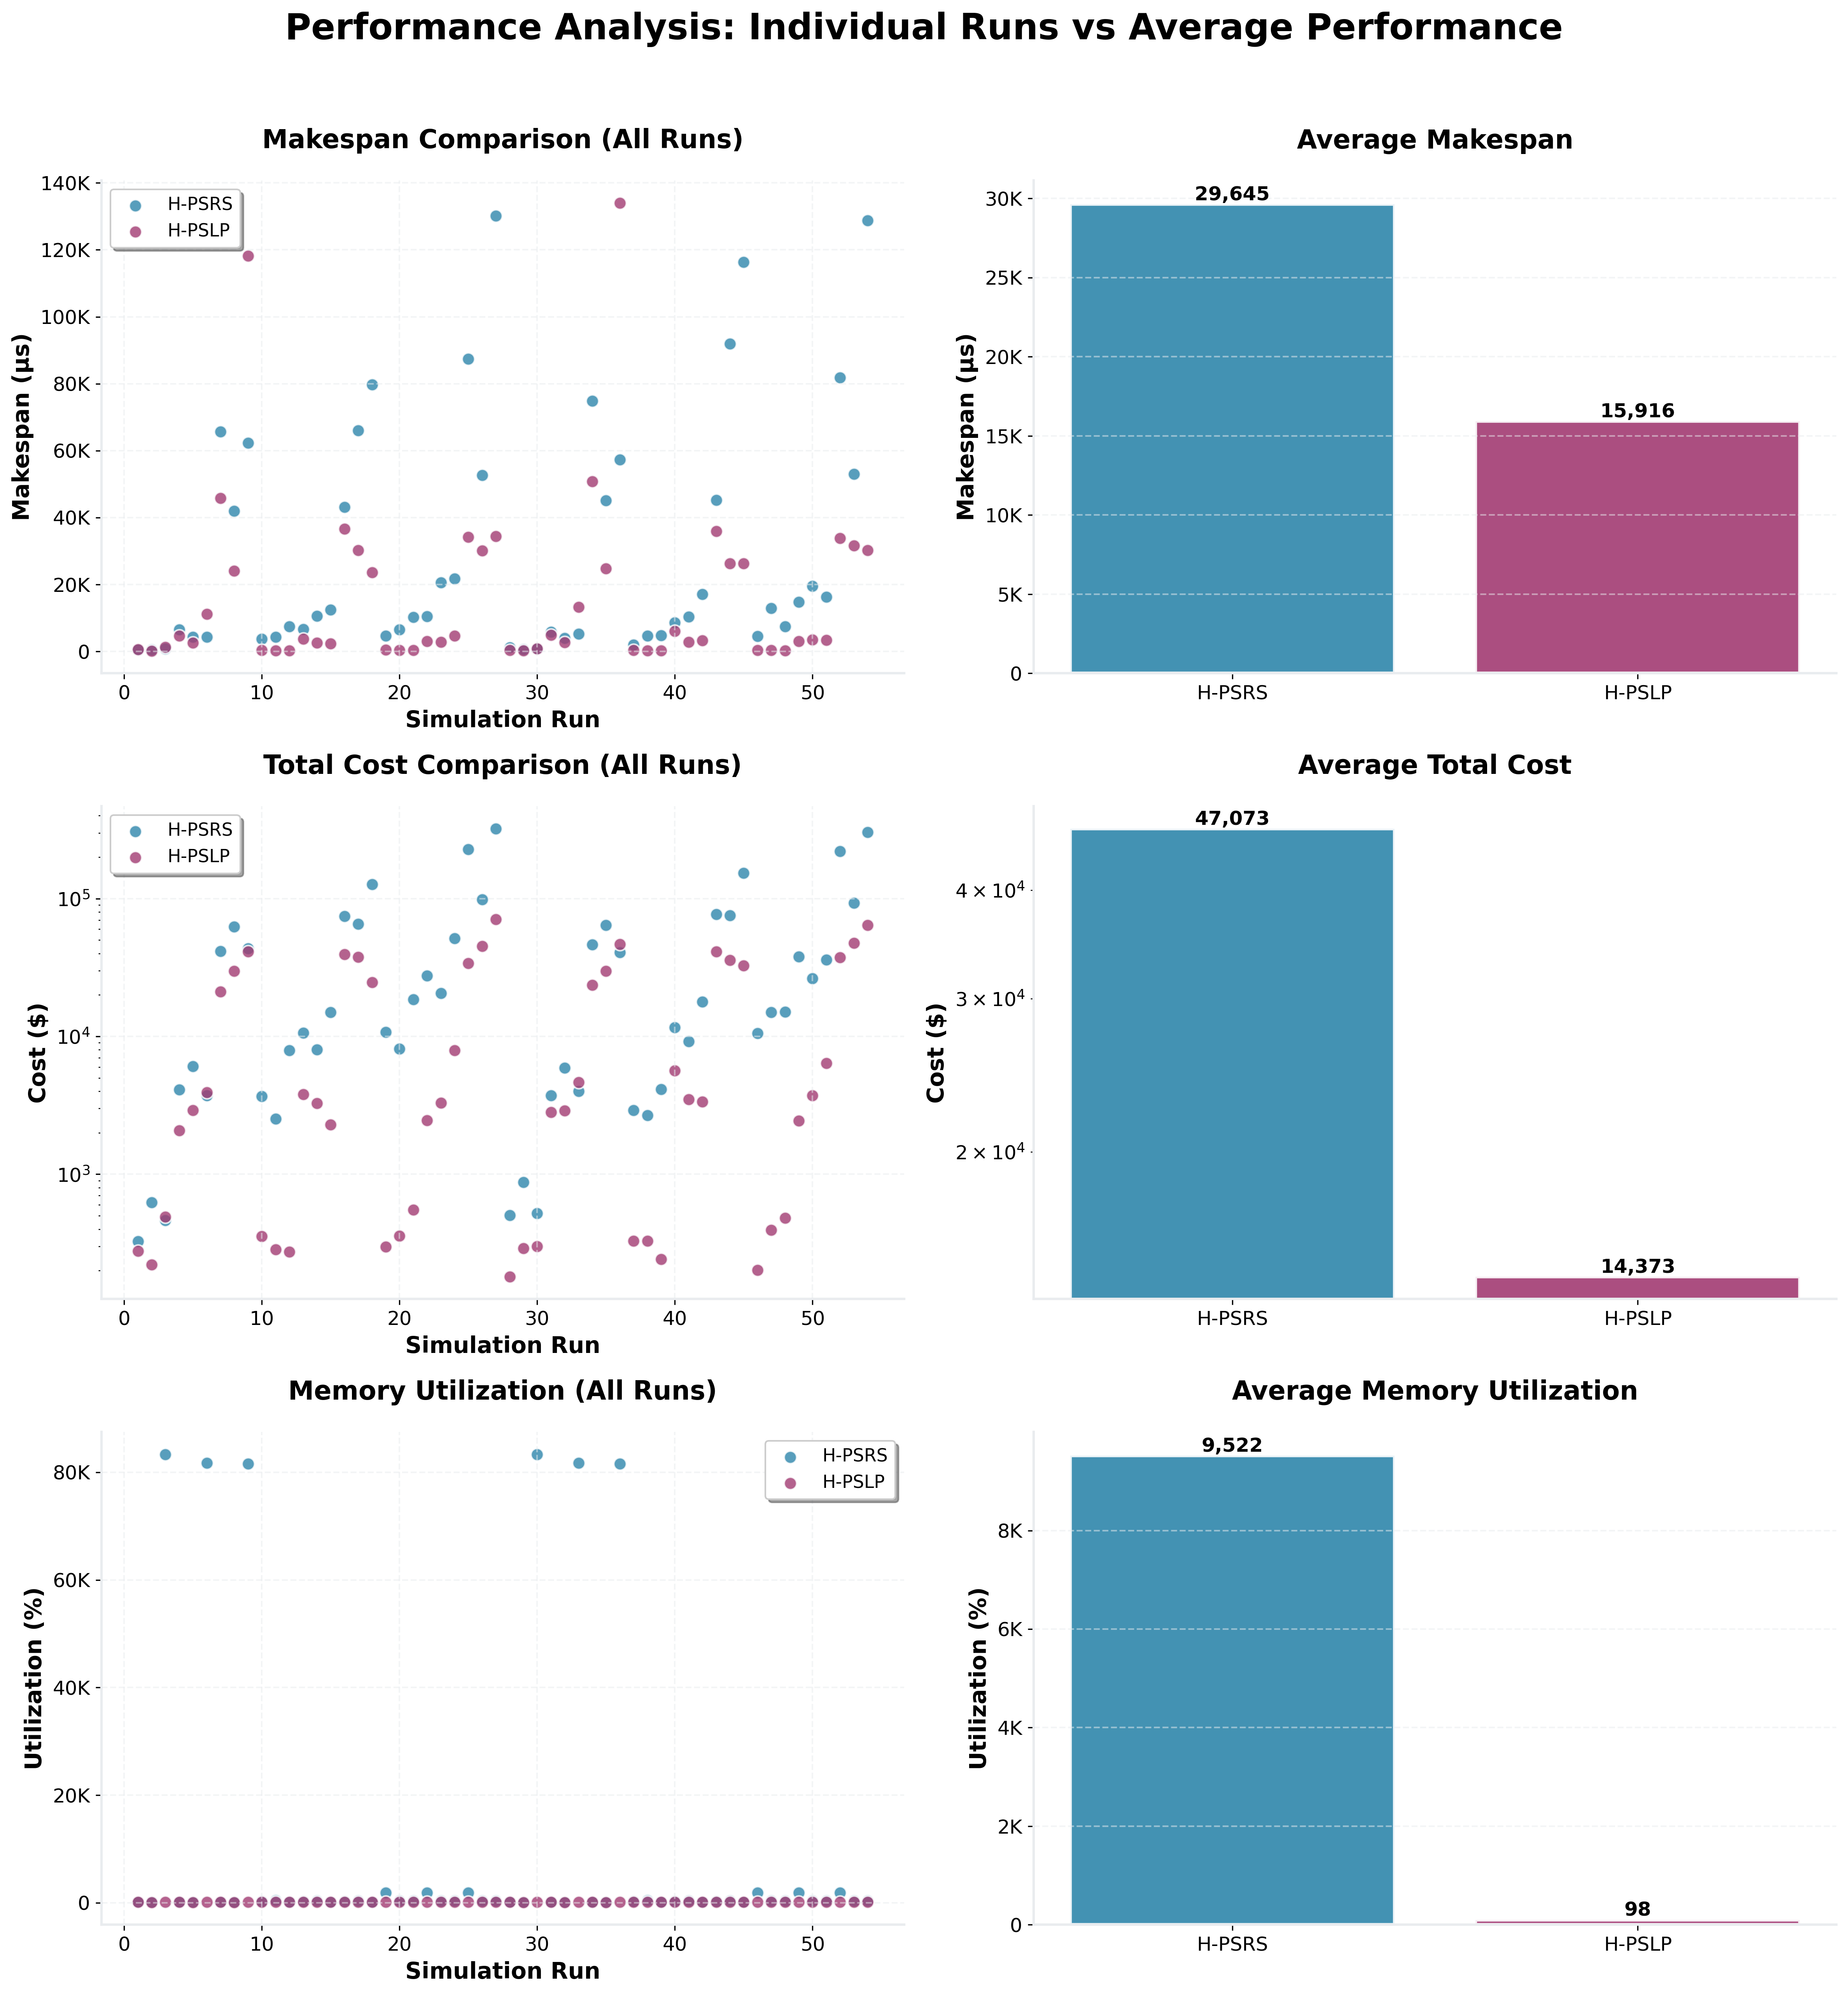
\includegraphics[width=1\linewidth]{images/agg_metrics_comparison.png}
    \caption{Overall Performance Comparison (Averaged Across All Runs)}
    \label{fig:overall_perf}
\end{figure}

On average, H-PSLP reduces the total execution time (makespan) by 46.3\% and the total operational cost by a remarkable 69.5\%. This efficiency stems directly from the LP model's ability to create a more globally aware data partition, minimizing the idle time that worker nodes experience while waiting for the most overloaded node to complete its sort. The most critical finding, however, lies in memory utilization. H-PSRS, which partitions data based on a simple throughput heuristic, is fundamentally memory-blind. This leads to catastrophic memory instability, with an average maximum peak utilization of over 9,500\% and a worst-case scenario (Run 3) reaching an untenable \textbf{83,330\%}. In a real-world system, this would result in consistent job failure. In contrast, H-PSLP maintains an average maximum utilization of 97.6\%. By design, it treats memory capacity as a hard constraint, ensuring that no node is ever assigned more data than it can handle. This architectural feature makes H-PSLP not only more efficient but also fundamentally more reliable.

\subsection{Scalability and Impact of Data Skew}

The performance gap between the two algorithms becomes more pronounced as the complexity of the sorting task increases, either through larger datasets or a greater number of nodes. To test the algorithms' robustness, we used a Gaussian (normal) distribution to introduce data skew, a condition that typically challenges simple partitioning schemes. The scalability analysis, presented in Figure~\ref{fig:scalability}, illustrates these trends.

% --- Figure 2: Scalability ---
\begin{figure}[h!]
    \centering
    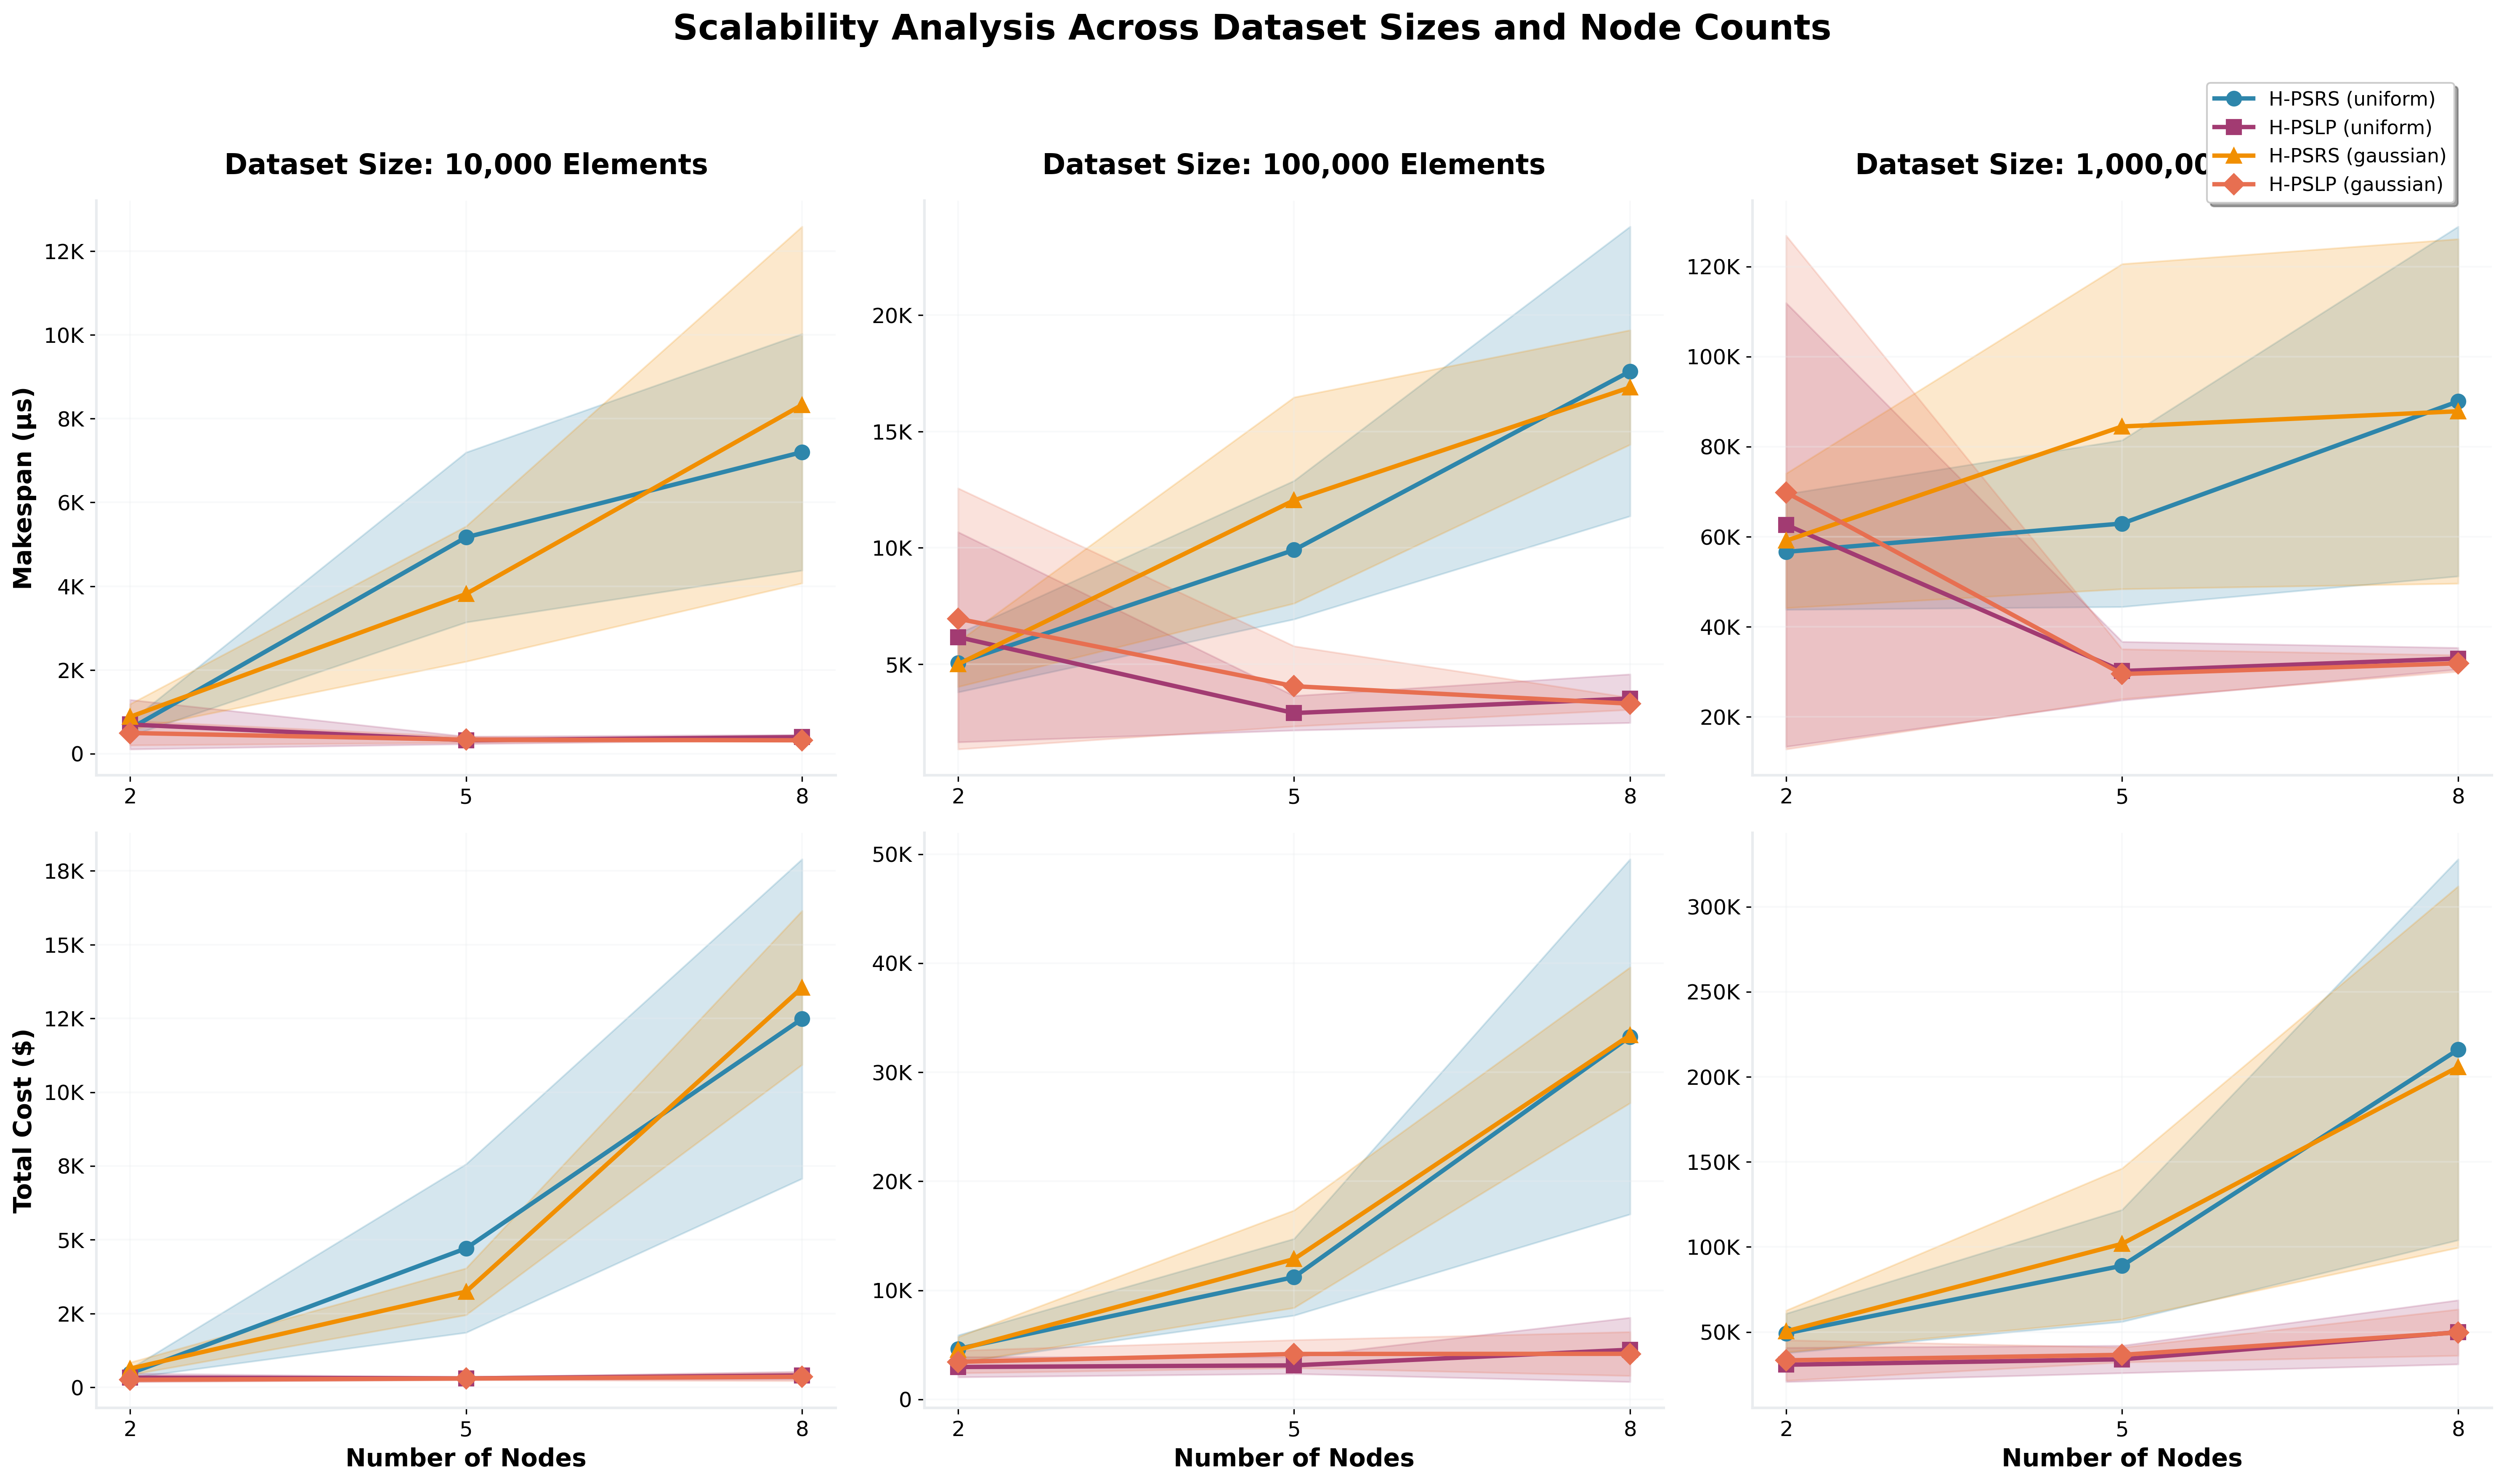
\includegraphics[width=1\linewidth]{images/scalability_analysis.png}
    \caption{Algorithm Scalability Analysis}
    \label{fig:scalability}
\end{figure}

As the dataset size grows from 10,000 to 1,000,000 elements, H-PSLP's makespan and cost advantages become increasingly dominant. H-PSRS, on the other hand, scales poorly. Its performance degrades significantly with more nodes, particularly when sorting the skewed Gaussian data. This occurs because its simplistic, throughput-based partitioning fails to account for the non-uniform data distribution, leading to severe load imbalance where a few nodes receive a disproportionate number of items to sort. The increased communication and synchronization overhead of managing more nodes exacerbates this problem, often resulting in worse performance with eight nodes than with five. H-PSLP, by contrast, demonstrates predictable and effective scalability, as its optimization model inherently balances the load regardless of the underlying data distribution. The visual difference between the uniform and Gaussian datasets, shown in Figure~\ref{fig:dataset_examples}, underscores the importance of this capability.

\subsection{Limitations and Architectural Trade-offs}

Despite its clear overall advantages, the performance data also highlights the architectural trade-offs and limitations inherent in the H-PSLP design. The most notable is the upfront computational overhead of the LP solver. While this cost is negligible for large-scale tasks, it can become significant for smaller, less complex workloads. This is evident in scenarios with specific node configurations and data distributions. For example, in Run 6 (uniform data, 100,000 elements, 2 nodes), H-PSRS achieved a much faster makespan (4,357 µs) compared to H-PSLP (11,239 µs). In such cases, the time invested in optimization does not pay off, and the simpler heuristic approach is more effective.

Furthermore, the LP model's predictive accuracy for the local sort phase, while strong, is not perfect. As shown in Figure~\ref{fig:lp_accuracy}, the model's predictions carry a Mean Absolute Percentage Error (MAPE) of approximately \textbf{29.9\%} for makespan and \textbf{23.3\%} for cost. This indicates that the partition generated is based on a highly effective, but ultimately heuristic, performance estimation. The immense overall performance gains affirm that this "good enough" optimization is far superior to the memory-blind approach of H-PSRS, but it is not a mathematically perfect global optimum for the true execution.

Finally, the current H-PSLP architecture retains a centralized merge phase, which presents a potential scalability bottleneck. While the parallel sort benefits from additional nodes, the final merge operation is sequential on the coordinator. As seen in Figure~\ref{fig:scalability}, the performance improvement of H-PSLP, while substantial, is not perfectly linear. This suggests that in massively parallel systems with a very large number of nodes, the final merge could become the dominant factor in the total makespan, limiting further speedup. This limitation highlights a clear direction for future work in exploring decentralized or hierarchical merge strategies.

% --- Figure 4: LP Accuracy ---
\begin{figure}[h!]
    \centering
    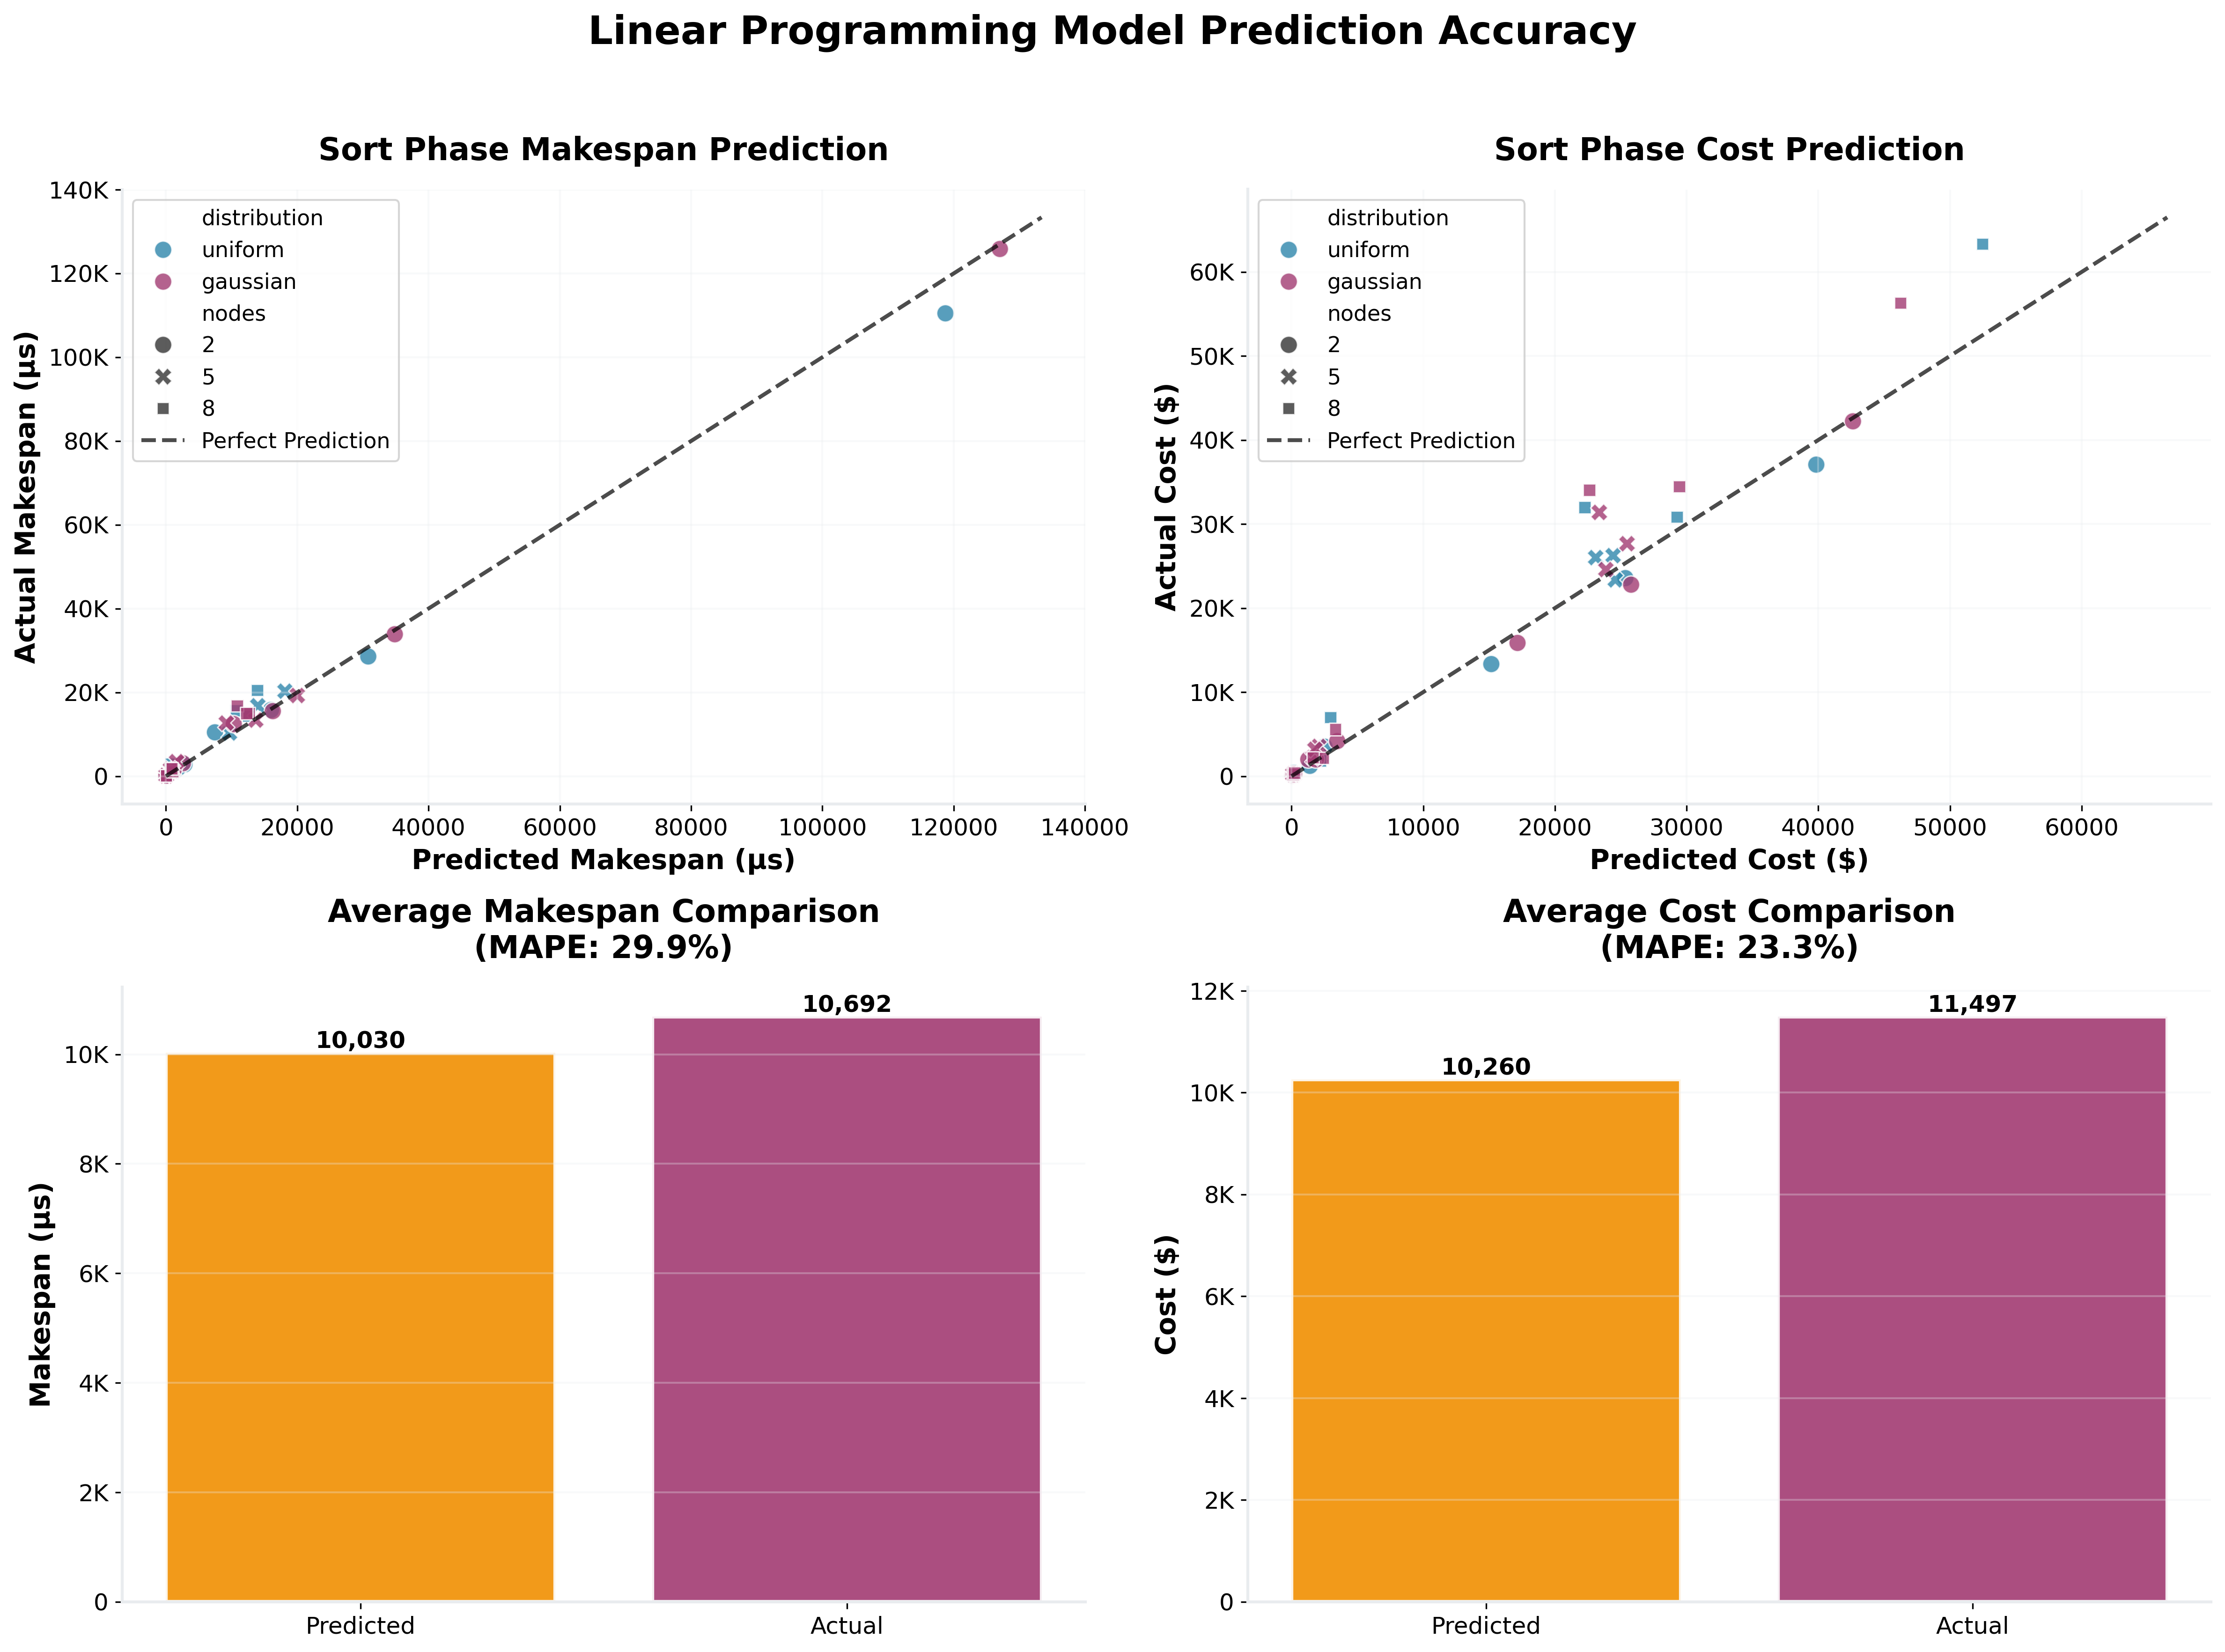
\includegraphics[width=1\linewidth]{images/lp_prediction_accuracy.png}
    \caption{H-PSLP Model Prediction Accuracy for Sort Phase (Averaged)}
    \label{fig:lp_accuracy}
\end{figure}


% --- Figure 3: Dataset Examples ---
\begin{figure}[h!]
    \centering
    \includegraphics[width=0.75\linewidth]{images/dataset_examples.png}
    \caption{Example Dataset Visualizations}
    \label{fig:dataset_examples}
\end{figure}



\section{Conclusion}

This work introduced and evaluated H-PSLP, a novel parallel sorting algorithm that integrates constrained linear programming to optimize data partitioning in heterogeneous environments. The experimental results demonstrate conclusively that this optimization-driven architecture is superior to the baseline H-PSRS across all key performance indicators. H-PSLP significantly reduces makespan (by 46.3\%) and operational costs (by 69.5\%) while, most critically, resolving the memory instability inherent in the H-PSRS approach. By treating memory as a hard constraint, H-PSLP guarantees system stability, preventing the catastrophic memory overflows observed in the baseline. We conclude that preemptive, model-driven data partitioning is a more robust and effective strategy for parallel sorting in heterogeneous systems than simpler, heuristic-based approaches.

\subsection{Applications}

The principles of H-PSLP are directly applicable to several real-world, large-scale data processing domains. In Cloud Computing and Big Data Analytics, it can optimize ETL jobs on heterogeneous virtual machine clusters, enabling faster and more cost-effective data preparation. For Scientific and High-Performance Computing (HPC), where clusters often consist of nodes from different hardware generations, H-PSLP can ensure that fundamental sorting tasks within complex scientific workflows are completed efficiently. Furthermore, its methodology can be adapted for Distributed Database Systems to optimize the sorting and aggregation of large, sharded result sets, thereby improving query response times.

\subsection{Future Work}

While this study validates the core premise of H-PSLP, the results also illuminate a clear path for future research. The first avenue is the development of an end-to-end LP model for the entire architecture. Our analysis of the LP model's accuracy (Figure~\ref{fig:lp_accuracy}) focused exclusively on the parallel sort phase, which it optimizes directly. A more holistic model would also incorporate the time and cost of the final centralized merge. This could enable more sophisticated trade-offs, potentially improving global makespan even if it requires a sub-optimal local sort.

This leads to a second area of investigation: exploring better merge strategies. The scalability analysis (Figure~\ref{fig:scalability}) shows that while H-PSLP's performance gains are substantial, they are not perfectly linear, suggesting the centralized merge can become a bottleneck at scale. Future work should investigate alternative topologies, such as hierarchical or decentralized peer-to-peer merging schemes, which could be integrated into an expanded LP model.

Finally, the crucial next step is to move beyond simulation and conduct an actual benchmark on a cloud platform. Deploying H-PSLP on a real-world heterogeneous cluster would provide the ultimate validation for the performance gains summarized in our results (Table~\ref{tab:agg_metrics}), allowing for the analysis of complex factors not modeled here, such as network latency and I/O contention, and confirming the algorithm's viability for production environments.





\printbibliography
\end{document}
